% !Mode:: "TeX:UTF-8"
% !TEX root = tjumain.tex

\iffalse
\bibliography{reference/reference.bib} % 欺骗latextools获取bib文件
\fi

%%%%%%% 正文 %%%%%%%

%%%% 引言 %%%%
\chapter{引言}
上世纪七十年代,“导电聚合物”的发现震惊了世界\cite{PhysRevLett.40.1472}。

\chapter{理论与计算方法}
\vspace{2mm}
\section{电子结构理论}
\vspace{2mm}
\vspace{2mm}
\subsection{Schrödinger方程和Born-Oppenheimer近似}
\vspace{2mm}
量子力学假设,微观粒子所处的状态可用波函数$\psi({\bf r},t)$进行表示,微观粒子在空间中分布的概率密度可用波函数的平方$|\psi({\bf r},t)|^2=\psi^*\psi$表示,波函数的时间演化遵循Schrödinger方程,Schrödinger方程的一般形式为\vspace{3mm}
\begin{equation}
    \label{eqn:sch_t}
\hat H \psi ({\bf r},t)=i\hbar\frac{\partial}{\partial t}\psi({\bf r},t) \vspace{3mm}
\end{equation}
每个可观测的力学量都对应一个线性厄米算符,如式~\eqref{eqn:sch_t}中的Hamilton算符$\hat H$就是一个这样的线性厄米算符。

Marcus理论中假设电荷转移反应具有如下特点:在发生电子转移反应前后,其对应的每个振动模式的力常数$k_j$不发生改变,那么对于反应物和产物而言,其能量和几何结构的关系可以用两个开口向上,二次项系数相同而顶点位置不同的抛物线进行表示,如图~\ref{fig:re}所示。

\begin{figure}[htbp!]
    \centering
    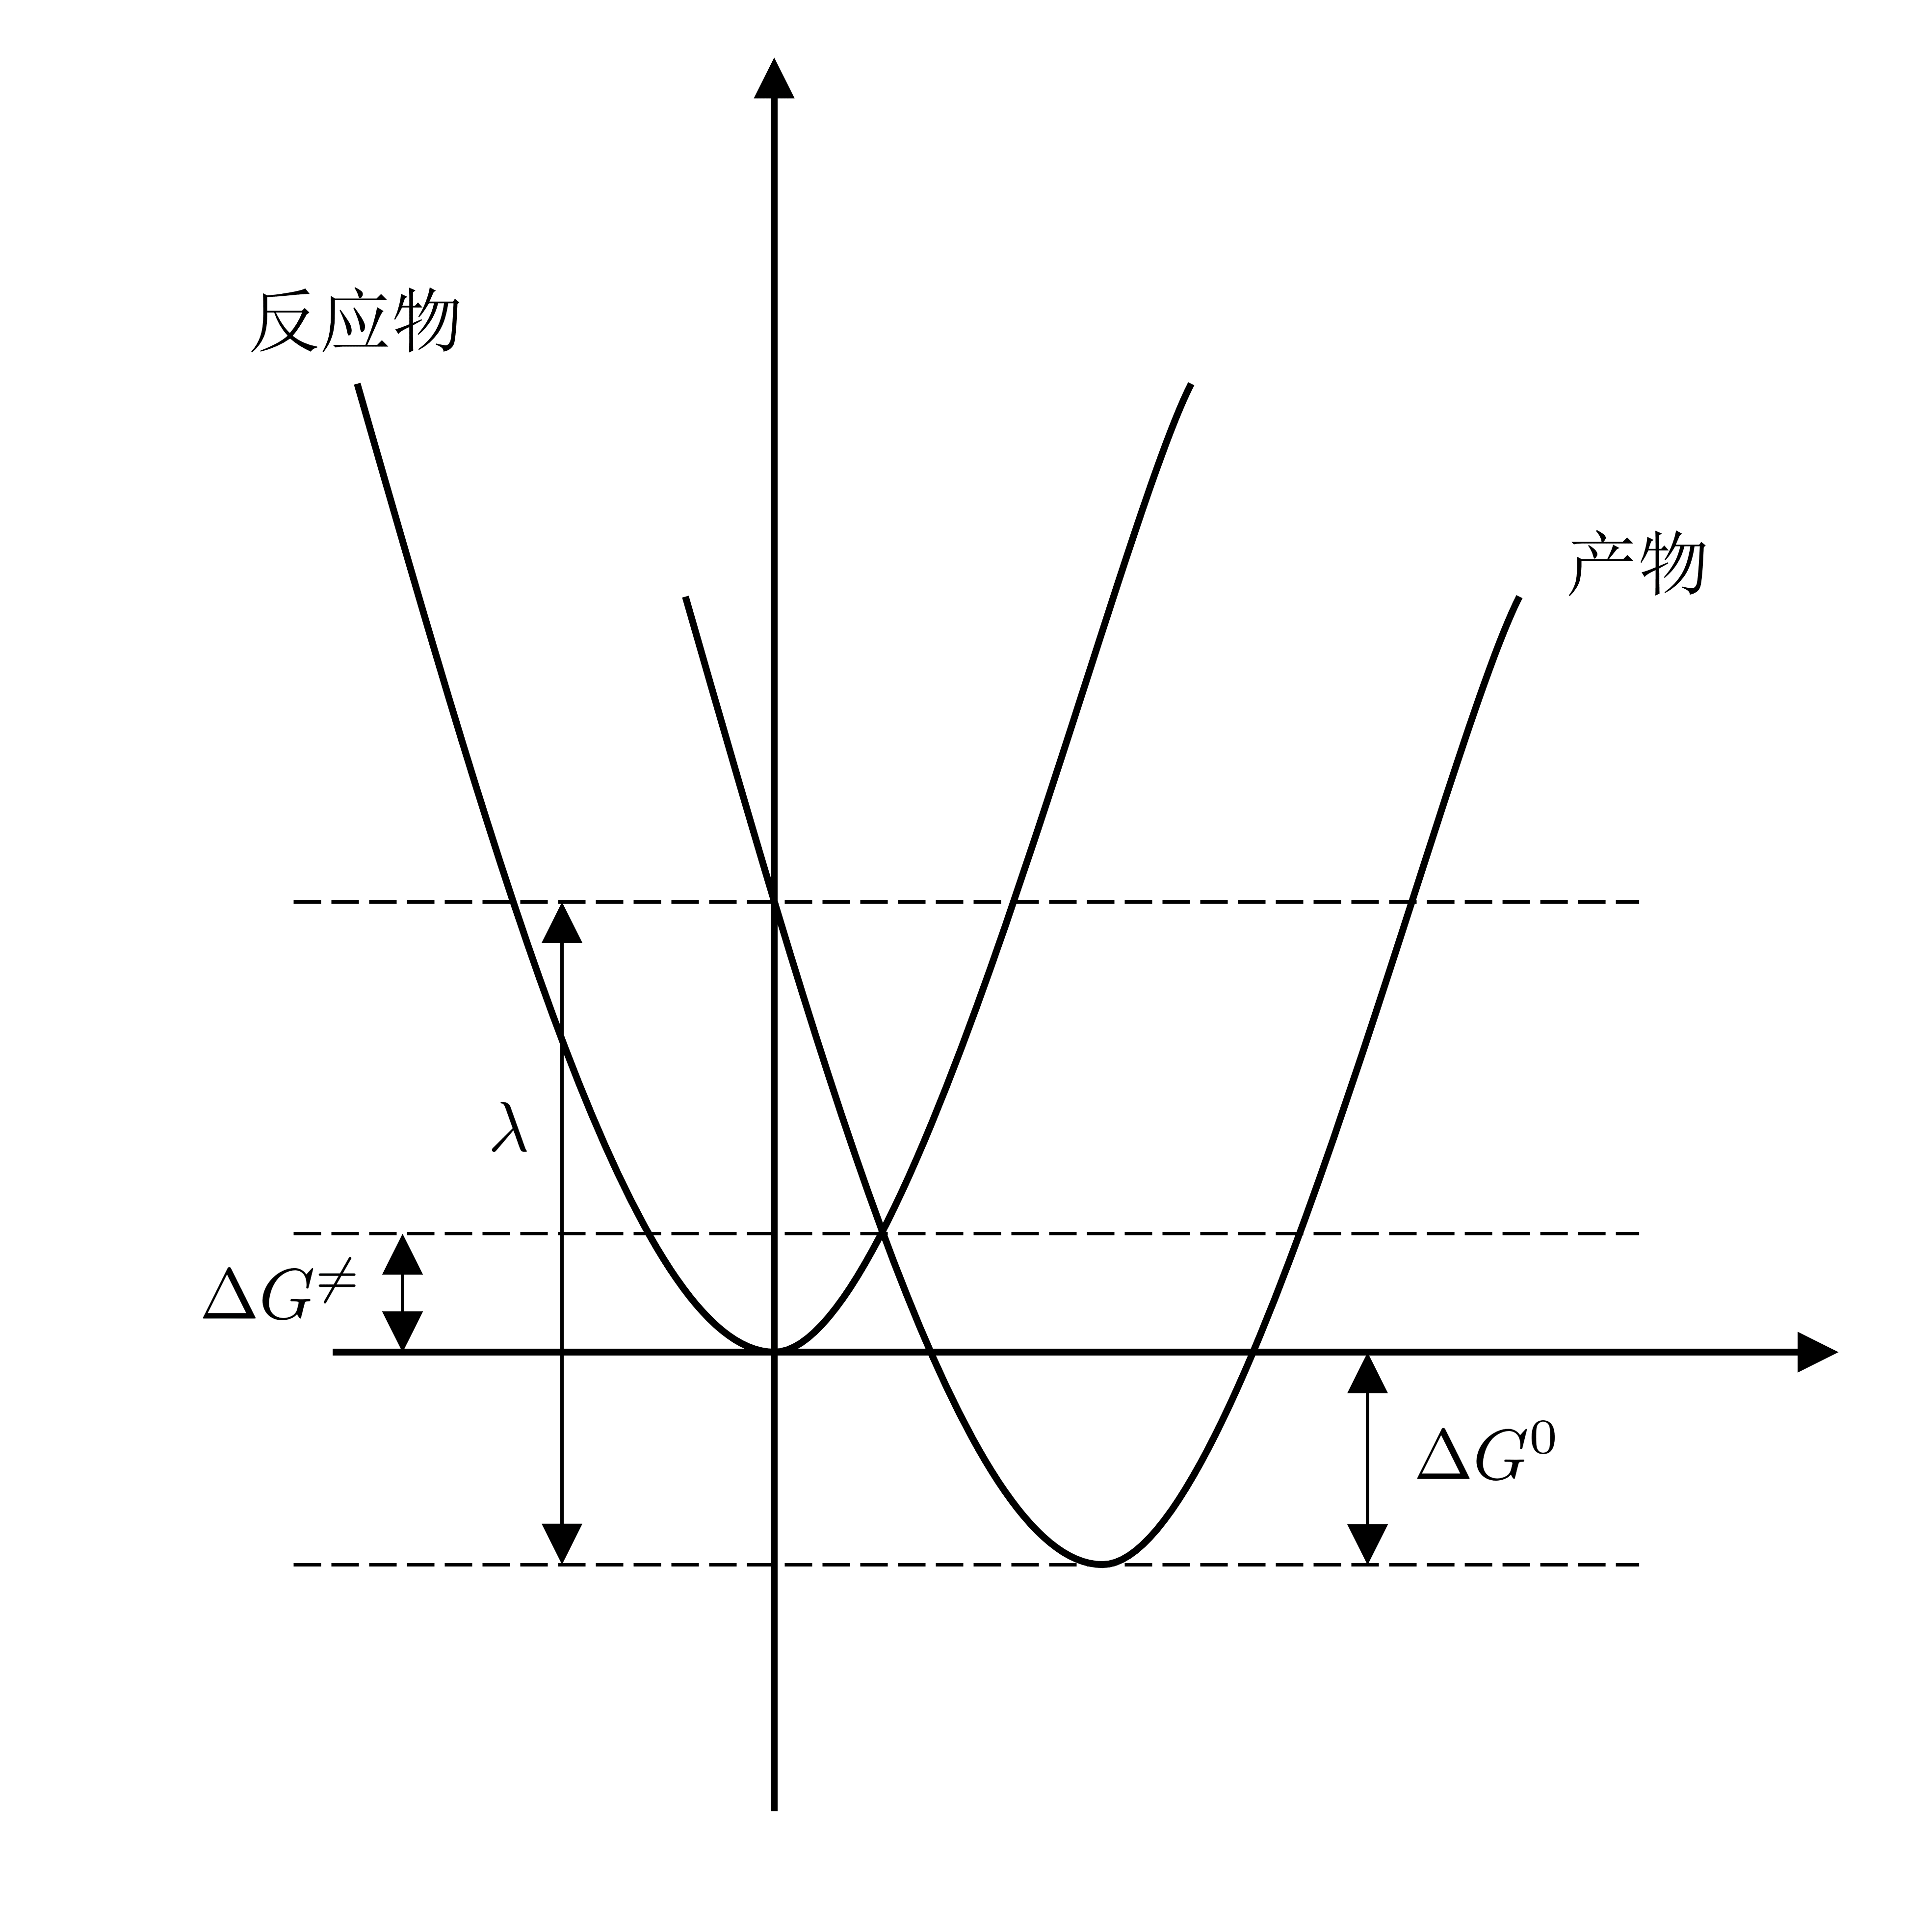
\includegraphics[width=0.5\textwidth]{re.png}
    \caption{重整能的计算示意图}\label{fig:re}
    \vspace{2mm}
\end{figure}

\chapter{结果与讨论}

%\chapter*{结\quad 论}
\chapter{总结与展望}

总结